\chapter{Conoscenze preliminari}
In questo capitolo descriveremo il funzionamento di FogMon (Sezione 2.1), le basi teoriche del Chaos Engineering (Sezione 2.2) e il progetto a cui fa riferimento il testbed su cui è stato distribuito FogMon in fase di verifica (Sezione 2.3).
    
    
    \section{Fogmon}
    Come menzionato nel Capitolo 1, FogMon è un prototipo, realizzato in C++, per il monitoraggio di infrastrutture Fog, in particolare delle risorse hardware (CPU, memoria, disco rigido), della QoS delle connessioni end to end (latenza, banda) e della presenza di dispositivi IoT nella rete \cite{FogMon}.
    
    
    FogMon può essere dispiegato su qualsiasi topologia di rete TCP/IP (previa configurazione) ed è costituito da due tipologie di componenti distribuite, ovvero i leader e i follower. I follower sono i responsabili delle misurazioni hardware e QoS e vengono assegnati a dei gruppi, ognuno dei quali fa riferimento a un leader. Un esempio di organizzazione di FogMon è illustrato in Figura \ref {fig:fogmon1}.
    
    \begin{figure}
        \begin{center}
            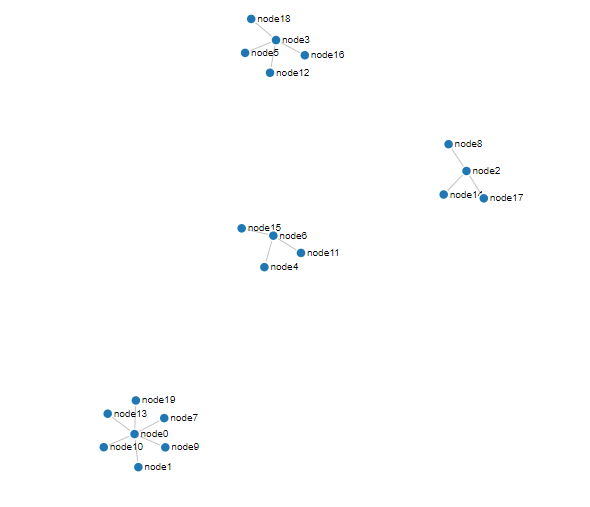
\includegraphics[width=10cm, height=10cm]{images/fogmon.PNG}
            \label {fig:fogmon1}
            \caption {Esempio di organizzazione di FogMon}
        \end{center}
    \end {figure}
    
    
    Attualmente FogMon è rilasciato come immagine Docker \cite{docker}; questo facilita l’installazione e l’esecuzione su qualsiasi macchina in grado di supportare container Docker e di gestire connessioni TCP/IP.
    
    FogMon orchestra diversi tool per raggiungere il suo scopo:
    \begin {itemize}
        \item Hyperic Sigar \cite{sigar} per il monitoraggio hardware e ICMP per la misura della latenza end-to-end (tramite ping)
        \item iperf3 \cite{iperf} ed Assolo \cite{assolo} per ottenere informazioni sulle prestazioni della banda (attivamente con iperf, passivamente con Assolo)
    \end{itemize}
    Leader e follower comunicano tra loro scambiandosi messaggi in formato JSON, sfruttando connessioni TCP. Ogni nodo archivia i dati e le misurazioni in un proprio database SQLite3.
    
    La flessibilità di FogMon risiede anche nella possibilità, per i nodi, di cambiare ruolo (da follower a leader e viceversa) e favorire la costruzione di una topologia migliore e più efficiente, in modo adattivo.
        \subsection{Follower}
        Essendo sviluppato per un ambiente Fog, FogMon assume che i nodi possano rapidamente entrare e uscire dalla rete su cui è distribuito. I follower, pertanto, possono effettuare connessioni e disconnessioni senza che queste operazioni impattino negativamente sul sistema.
        
        
        La topologia di Fogmon viene costruita sulla base di un criterio di prossimità, per cui ogni follower viene assegnato al gruppo del leader verso il quale ha la minima latenza \textit{end-to-end}; quando un nodo si unisce all’ambiente monitorato da FogMon (come follower), conosce inizialmente solo l’indirizzo del leader specificato nella configurazione iniziale. Il nodo a cui si connette il follower agirà da intermediario per fornire la lista degli altri leader a cui il follower potrebbe connettersi.
        
        
        Da qui, il follower eseguirà delle misurazioni della latenza verso ognuno dei leader appena reperiti per connettersi al nodo che presenta il valore più basso, garantendo così il rispetto del criterio di prossimità. i follower cercano sempre il leader con la latenza minore: questo processo di divisione dà origine ai gruppi, ovvero insiemi di follower sotto lo stesso leader. Il processo appena descritto vale anche nel caso in cui un follower non riesca più a raggiungere il proprio leader o nell’eventualità in cui, tramite controlli periodici, un follower individui un leader migliore di quello attuale. 
        
        
        Un altro aspetto importante si identifica nel processo di misurazione della larghezza di banda, eseguito dal nodo Follower, per capirne il livello di affidabilità; FogMon, come accennato, utilizza due sistemi di rilevazione della banda:
        \begin{itemize}
            \item Iperf3, un sistema di rilevazione attiva e, pertanto, intrusiva \cite{iperf}
            
            \item Assolo, un sistema di rilevazione passiva, ma meno affidabile \cite{assolo}
        \end{itemize}
        Per combinare il meglio dei due strumenti, FogMon si ispira al modello ibrido di Marttinen et al. \cite{marttinen}, che riduce a un terzo il numero di misurazioni attive e, pertanto, diminuisce l'intasamento della banda mantenendo comunque dati validi.
        
        Per ridurre ulteriormente il sovraccarico di rete, FogMon invia dati di monitoraggio sia hardware che QoS (uso dela CPU e della memoria, traffico in entrata e uscita, latenza), da follower a leader, basandosi su un sistema di aggiornamenti differenziali. In dettaglio, i follower ripetono la comunicazione di dati comparabili a quelli già misurati e inviati precedentemente, ma solo quelli la cui media o varianza dei valori del report, se confrontata con quelli del report precedente, differisce più di una soglia impostata (ovvero 10\% per impostazione predefinita) dall'ultimo aggiornamento eseguito. Vista la necessità di ridurre lo spazio di archiviazione sfruttato da FogMon, solo le ultime 30 misurazioni vengono conservate nel database di ciascun nodo.\\
        \subsection{Leader}
        FogMon organizza il proprio overlay in modo che il numero dei leader sia pari alla radice del numero totale dei nodi, approssimata all'intero successivo.
        
        
        I nodi leader sono responsabili dell’aggregazione dei dati ricevuti dai follower come risultato del loro monitoraggio. Si occupano inoltre dell’organizzazione della topologia peer-to-peer basandosi sulle metriche misurate dagli altri nodi e sulle informazioni reperite mediante le operazioni di “gossiping” \cite{jelasity}, ovvero lo scambio di dati tra i leader. Ogni leader effettua il monitoraggio del nodo su cui è in esecuzione. I leader raccolgono i dati dai follower che monitorano, i quali riportano periodicamente i dati che misurano.
        
        Infine, ogni leader riesce, tramite la comunicazione con gli altri leader (gossiping), a memorizzare i dati dei follower di altri gruppi.
        
        
        Ad ogni lasso di tempo stabilito, ogni Leader seleziona un altro Leader casuale e invia un report completo sul proprio gruppo di Follower. In aggiunta, il Leader ignora qualsiasi follower che risulti disconnesso, ossia che non ha inviato report negli ultimi due heartbeat. I valori di latenza e banda vengono stimati dai leader \cite{FogMon}, basandosi sull'assunzione che le tecnologie di accesso a Internet (ad esempio, xDSL, 3G, 4G) siano asimmetriche e rappresentino un collo di bottiglia nella comunicazione, specialmente tra i nodi che risiedono ai margini di Internet.
        \subsection{Ricalcolo della topologia}
        FogMon è in grado di decidere autonomamente e adattivamente quali siano i nodi più indicati (in base alle misurazioni di latenza tra i nodi) per agire da leader e come organizzarli in gruppi. Per garantire l'accuratezza delle stime di banda e latenza tra gruppi diversi, FogMon può ristrutturare l'overlay peer-to-peer tra Leader e Follower.
            La ristrutturazione della topologia di rete viene eseguita quando:
            \begin{itemize}
                \item la dimensione della rete raddoppia (o dimezza) rispetto all'ultima ristrutturazione, il che implica che più (o meno) Leader dovrebbero essere designati per gestire la complessità del monitoraggio
                
                \item la qualità del raggruppamento misurata tramite l'indice di Davies-Bouldin \cite{davies-bouldin} (rapporto tra la latenza intergruppo e intragruppo) della topologia corrente supera un parametro soglia, selezionata a 3 per impostazione predefinita.
            \end{itemize}
        Ogni volta che un Leader scopre che una delle due condizioni vale, viene avviata una procedura per il ricalcolo della topologia di FogMon; più leader, anche  contemporaneamente, possono avviare questa procedura.
        
        I leader che ricevono la richiesta, ma non ne hanno iniziata una a loro volta, si limitano a riconoscere il nodo che avvia la procedura; eventuali altri leader che hanno avviato la richiesta, invece, dovranno confrontarsi per trovare il nodo incaricato di gestire il processo di ristrutturazione della topologia.
        
        A questo punto, il leader che guida il ricalcolo invia un messaggio di avvio a tutti gli altri leader, che iniziano a elaborare
        una nuova topologia candidata, sfruttando l'algoritmo k-medoids \cite {k-medoids}. Ogni Leader coinvolto propone una soluzione (e una valutazione sulla qualità di questa soluzione), che verrà candidata come possibile nuova topologia. 
        
        Tutti i nodi che devono cambiare ruolo svolgono questa operazione prima dell'avvio del nuovo overlay della rete; i nuovi leader attendono quindi il termine di tutti cambiamenti di ruolo. I follower, invece, sfruttano le informazioni raccolte durante il ricalcolo della topologia per selezionare il leader più vicino ad essi.
        
        
        \subsection{FogMonEye}
        FogMonEye \cite{FogMonEye} è un microservizio REST sviluppato specificamente per FogMon nell'ambito dell'esperimento LiSCIo \cite{FogMon}. Può essere ospitato su un server esterno, il suo compito primario è quello di collezionare i risultati degli esperimenti effettuati, rendendoli disponibili tramite API REST e un'interfaccia grafica web.
        
        FogMonEye raccoglie i dati che riceve dai nodi leader e li confronta con la topologia impostata inizialmente per configurare l'esperimento. Tale operazione permette di calcolare i seguenti dati: 
        \begin{itemize}
            \item L'errore relativo sulle stime di banda e latenza nei gruppi
        
            \item L'errore relativo sulle stime di banda e latenza tra gruppi
        
            \item Il consumo di risorse in un determinato lasso temporale (uso massimo, minimo e medio di CPU, Memoria e banda)
        
            \item Il tempo necessario per riorganizzare l'overlay di FogMon dopo un cambio dell'infrastruttura, causato da una ristrutturazione della topologia 
            
            \item Una rappresentazione grafica dell'attuale overlay di topologia di FogMon, suddiviso in gruppi 
        \end{itemize}
        I dati appena elencati, ad eccezione dell'ultimo, vengono organizzati in fasi dell'esperimento (dette ``momenti"). La figura \ref{fig:Eye} mostra un esempio di resoconto di un esperimento monitorato da FogMonEye.
        \begin{figure}
        \begin{center}
            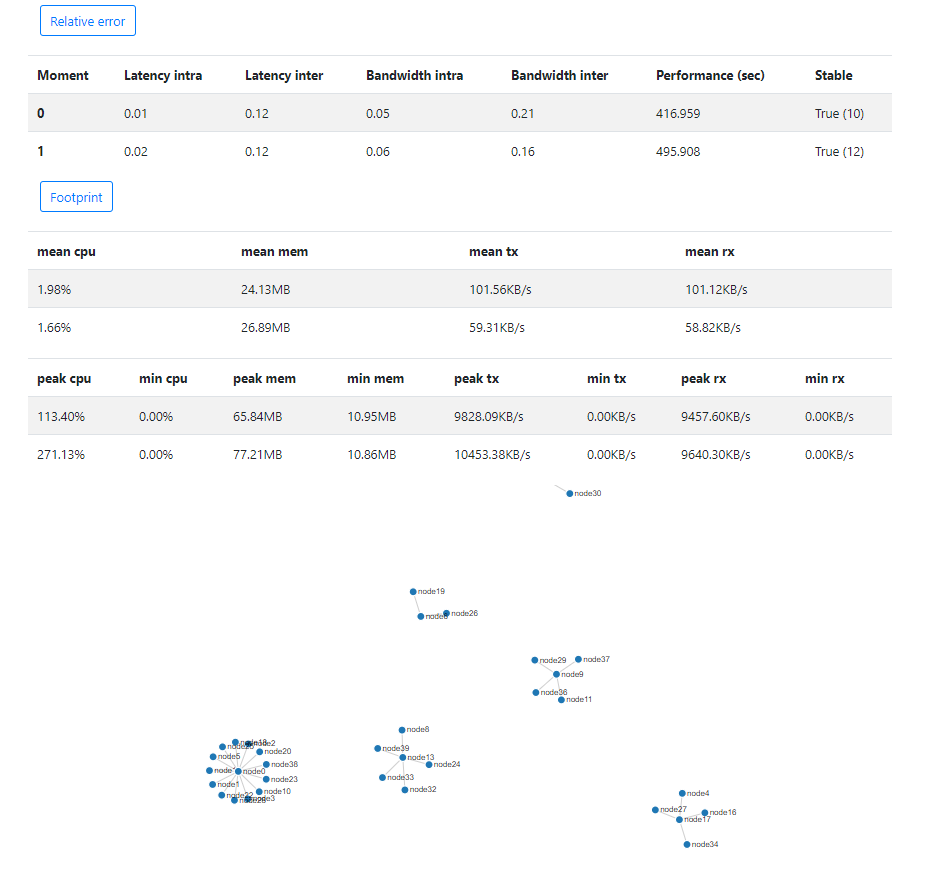
\includegraphics[width=15.6cm, height=13.4cm]{images/Eye.PNG}
            \label {fig:Eye}
            \caption {Esempio di esperimento monitorato da FogMonEye}
        \end{center}
        \end {figure}
        
        
        FogMonEye permette anche di monitorare più esperimenti contemporaneamente e di conservare, al termine, i risultati. Ogni esperimento viene identificato da un ID di sessione, determinato inizialmente tramite l'invio di una specifica a FogMonEye. Per ogni sessione è possibile, inoltre, accedere mediante richieste http a tutti i dati raccolti.
    \newpage
    \section{Chaos Engineering}
    Il Chaos Engineering \cite{princofchaos}\cite{gremlinchaos} è un insieme di tecniche di testing volto a ricercare errori nel sistema mediante l’iniezione volontaria e programmata di fallimenti, in modo da controllare la reazione e possibilmente aumentare la resilienza del sistema di fronte a tali eventi. Questo permette di rivelare comportamenti del programma altrimenti non identificabili, di prevederne le conseguenze sugli utenti e di risolvere tali mancanze il prima possibile.
    
    L'uso del chaos engineering non deve essere sostitutivo delle classiche metodologie di testing, quanto un'integrazione che si rivela particolarmente utile in sistemi che basano il proprio funzionamento su nodi interconnessi \cite{queue}. La caratteristica del testing classico è quella di avere un input e un output già previsti, pertanto non genera alcuna conoscenza completamente nuova su come si comporterà il sistema se dovesse verificarsi un fallimento. Al contrario, con il chaos testing si eseguono esperimenti più ampi, per simulare anomalie infrastrutturali non pianificate. Tutto ciò consente di ottenere nuove conoscenze sui comportamenti, le proprietà e le prestazioni del sistema.
    
   Tra i pionieri del Chaos Engineering troviamo Netflix, che nel 2011 ha proposto Chaos Monkey \cite{Netflix}. Si tratta di uno strumento per testare la resilienza della sua infrastruttura IT. Funziona disabilitando intenzionalmente i server nella rete di produzione di Netflix per testare come i sistemi rimanenti rispondono all'interruzione. L'origine del nome ``Chaos Monkey" è spiegata in \cite{Martinez}:
    
    \emph{``Immagina una scimmia che entra in un `data center', queste `fattorie' di server che ospitano tutte le funzioni critiche delle nostre attività online. La scimmia strappa i cavi in modo casuale, distrugge i dispositivi e getta tutto ciò che trova. La sfida per i responsabili IT è progettare il sistema informativo di cui sono responsabili in modo che possa funzionare nonostante queste scimmie, che nessuno sa mai quando arriveranno e cosa distruggeranno "}.
    
    Dopo Netflix, la necessità di costruire un sistema resiliente e pronto a reagire ai guasti sta spingendo molte altre aziende ad adottare il chaos engineering. Realtà come Amazon \cite{amazon}, Google \cite{Google} e Facebook \cite{Facebook} stanno già adoperando queste tecniche per migliorare i loro sistemi distribuiti, o parti di essi.
    Un altro esempio è da ricercare nella National Australia Bank \cite{NAB}, anch’essa pioniera nello sviluppo di sistemi con l'aiuto del Chaos Engineering. 
    
    
    Il Chaos Engineering può aiutare a identificare errori di disegno di un software distribuito, dovuti a un ampio insieme di assunzioni errate da parte degli sviluppatori \cite{miles}, ad esempio:
    \begin{itemize}
        \item La rete non presenta punti deboli, latenze elevate o problemi di banda
        
        \item La topologia non muta nel tempo
        
        \item I costi di manutenzione e le risorse necessarie alla comunicazione sono identici tra implementazioni diverse 
        
        \item Il sistema è sorvegliato da un amministratore 
        
        \item La potenza di calcolo dei dispositivi non è un problema 
    \end{itemize}
    Tali ipotesi chiaramente non sono da considerare valide nello sviluppo di un’architettura software distribuita, dispiegata su una rete reale, composta da dispositivi fallibili e soggetti a possibili errori di rete.
        \subsection{Esperimento di chaos}Di seguito si riporta il metodo di creazione degli esperimenti di chaos, a partire dalla formulazione dell’ipotesi fino alla sua verifica \cite{miles}\cite{jones} .
        
        Un esperimento di \textit{Chaos Engineering} prevede la creazione di una \textit{Steady State Hypotesis} (ipotesi di stato stabile) e una prima verifica di questa ipotesi per confermare la stabilità del sistema. In seguito, si applica un ``metodo" (fallimento che può compromettere l'ipotesi) e si esegue una seconda verifica della \textit{Steady State Hypotesis}, al fine di identificare, se c'è stata, una deviazione. Possiamo riassumere l'iter appena descritto per un esperimento di \textit{Chaos Engineering} con la figura \ref{fig:5-6miles}.
        \begin {figure}
        \begin{center}
            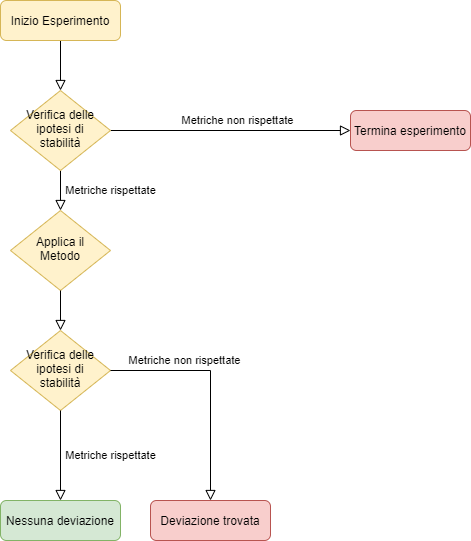
\includegraphics[width=11cm, height=13cm]{images/56miles.png}
            \caption {Passaggi di un esperimento di chaos engineering}
            \label{fig:5-6miles}
        \end{center}
        \end {figure}
        Se al termine della procedura si osserva che l'ipotesi non è rispettata, siamo di fronte a un errore del sistema. In questo caso è necessario ripristinare le condizioni precedenti all'esperimento e implementare una soluzione per evitare che si verifichi nuovamente.
        Nel seguito sono spiegati in dettaglio le fasi di creazione dell'ipotesi e del metodo, di raccolta e di analisi dei dati e di verifica delle ipotesi.
        \subsection{Creazione dell’ipotesi e del ``metodo"}
        È importante, come prima cosa, definire delle metriche per descrivere il funzionamento del sistema, ovvero che alcune assunzioni stabiliscano quale sia il comportamento corretto del software. Parliamo, in questo caso, di \emph{steady state hypotesis}, ossia di ipotesi di funzionamento del sistema in condizioni di stabilità. Secondo \cite{miles}:
        
        
        \emph{``l'ipotesi [dello steady state] esprime, entro determinate tolleranze, ciò che costituisce normale per la parte del sistema testata dall'esperimento di Chaos}.
        
        
        Le ipotesi create definiscono i “limiti” delle azioni che il software dovrebbe poter effettuare e, quindi, modellano quale debba essere il suo funzionamento. Tali ipotesi sono verificabili tramite dei parametri misurabili (ed eventualmente soggetti a una certa tolleranza).
        
        L'applicazione del chaos engineering richiede la verifica di tutte queste ipotesi, per identificare la condizione di stabilità prima e dopo l'iniezione di fallimenti infrastrutturali. Tipicamente le \textit{steady state hypotesis} indicano i comportamenti attesi in merito all’integrità e validità dei dati dell’applicazione, ai tempi delle risposte del sistema all’utente. Prendendo ad esempio Netflix, la società utilizza la velocità con cui i clienti premono il pulsante di riproduzione su un dispositivo di streaming video come parametro, definendo questa metrica come ``flussi al secondo" \cite {cheatsheet}.
        
        
        Il metodo di un esperimento di Chaos definisce le azioni che influenzeranno il sistema e causeranno le condizioni turbolente (ossia il caos) che dovrebbero essere applicate al sistema di destinazione.
        
        
        I fallimenti iniettati quindi non sono, come suggerirebbe il nome “chaos”, casuali. La formulazione di un’ipotesi comporta la ricerca e lo studio di tutti gli scenari che potrebbero portare al fallimento di essa o di altre ipotesi; pertanto, per ogni Steady State Hypotesis verranno realisticamente pensati più metodi per testare più scenari (ad esempio la degradazione della QoS di rete, il crash di un nodo, un errore software).
        
        
        L’iniezione del fallimento deve essere controllabile ed osservabile in modo che la reazione del sistema sia identificabile nel guasto provocato e, pertanto, rimediabile in caso di comportamenti indesiderati. Questa fase deve chiaramente essere effettuata sotto controllo, previo backup del sistema, per evitare che avvengano danni irreversibili al sistema su cui viene eseguito il test, o ai dati del software stesso, e deve essere accompagnata da una strategia di ripristino definita come \textit{rollback} \cite{miles}. Ciò è realizzabile in due tipologie di ambienti:  
        \begin{itemize}
            \item un testbed, dove l'esecuzione del software è puramente a fini di prova e pertanto un eventuale guasto non comporta danni all’infrastruttura o ai dati di un sistema vero e proprio. In questo caso non è necessario un punto di ripristino né una strategia di \textit{rollback}, oppure 
            \item un ambiente di produzione controllato, presumibilmente già più resistente ai fault, con un backup dei dati e misure di sicurezza per l’hardware, accompagnati dalla strategia di rollback per evitare di danneggiare un sistema in funzione.
        \end{itemize}
        Alle due possibilità appena elencate, è possibile affiancare una metodologia CI/CD (continuous integration/continuous delivery) per creare un flusso di integrazione e distribuzione continuo, particolarmente utile nelle fasi di integrazione e test \cite{cicd}.
        \subsection{Analisi dei dati e verifica delle ipotesi}
        La raccolta delle risposte, da automatizzare laddove le metriche di riferimento siano molteplici, deve essere seguita dalla loro analisi. L'analisi consiste principalmente nel verificare tutte le \textit{steady state hypotesis} formulate sul corretto funzionamento del programma. Tale passaggio è importante perchè se si riscontrano deviazioni dalle condizioni attese è stata identificata una potenziale debolezza del sistema.
        
        Come menzionato precedenemente, l'ipotesi dello stato stazionario viene utilizzata due volte: una volta all'inizio dell'esecuzione dell'esperimento e poi di nuovo quando il metodo dell'esperimento ha completato la sua esecuzione:
        \begin{itemize}
            \item All'inizio dell'esecuzione di un esperimento, viene valutata l'ipotesi per decidere se il sistema in oggetto è in uno stato stabile. Se il sistema target si discosta dalle aspettative dell'ipotesi a questo punto, l'esperimento deve essere interrotto, poiché non ha alcun valore dato che il sistema non è riconoscibilmente stabile sin dall'inizio.
            \item Il secondo utilizzo dell'ipotesi dello stato stazionario costituisce il suo ruolo principale nell'esecuzione di un esperimento. Dopo l'applicazione del metodo, la \textit{Steady state hypotesis} viene nuovamente confrontata con il sistema bersaglio. Questo è il punto critico dell'esecuzione di un esperimento, perché rappresenta il momento in cui si possono identificare delle deviazioni, che rischiano di presentarsi nuovamente nel caso in cui il sistema sia sottoposto a condizioni simili a quelle causate dal metodo.
        \end{itemize}
        \paragraph{Chaos Cards}
        In \cite{miles} si descrive come per ogni esperimento sia possibile riassumere le componenti principali in \textit{Chaos Cards}, ovvero un'istanza di \textit{Chaos Experiment} che include:
        \begin{itemize}
            \item La \textit{Steady State Hypotesis}
            \item Le metriche di verifica delle ipotesi (ossia lo spettro di valori accettabili su parametri misurabili)
            \item Il metodo da applicare
            \item Il piano di \textit{Rollback} in caso di deviazione
        \end{itemize}

    \section{Fed4Fire+ e JFed}
    Come accennato nel Capitolo 1, la sperimentazione si è svolta nell'ambito del progetto LiSCIo \cite{FogMon}, il cui scopo è quello di testare e mettere a punto FogMon sfruttando le risorse fornite da Fed4Fire+.
    
    
    Fed4FIRE + è un progetto nell'ambito del programma Horizon 2020 dell'Unione Europea, che offre una federazione di testbed Next Generation Internet (NGI) \cite{Fed4Fire+}.
    
    
    Con le risorse fornite da Fed4Fire+, LiSCIo mira a rendere FogMon in grado di gestire le variazioni nella rete su cui è distribuito, insieme ai possibili fallimenti dei nodi da cui la rete stessa è composta.
    
    
    Fed4Fire+ mette a disposizione vari strumenti per facilitare le sperimentazioni. Tra questi  Jfed \cite{jfed}, un software basato su Java per l'uso di testbed. Tale strumento utilizza un sistema di credenziali e di certificati per autenticare e autorizzare gli utenti su questi testbed. L'utente può creare nuovi esperimenti trascinando da un'area di selezione i tipi di nodi che intende utilizzare.
    
    
    In Figura \ref{fig:jfed} vediamo un esempio di esperimento creato tramite l'interfaccia di Jfed: dopo aver trascinato alcuni nodi, l'utente può selezionare su quale banco di prova desidera eseguire l'esperimento. È possibile eseguire una configurazione aggiuntiva come la selezione di un nodo specifico, la modifica del funzionamento predefinito sistema e selezionare uno script da eseguire all'avvio del nodo. È possibile anche tracciare connessioni di rete tra i nodi; questa operazione causerà la creazione di una VLAN all'interno del testbed prescelto.
    \begin {figure}
    \begin{center}
            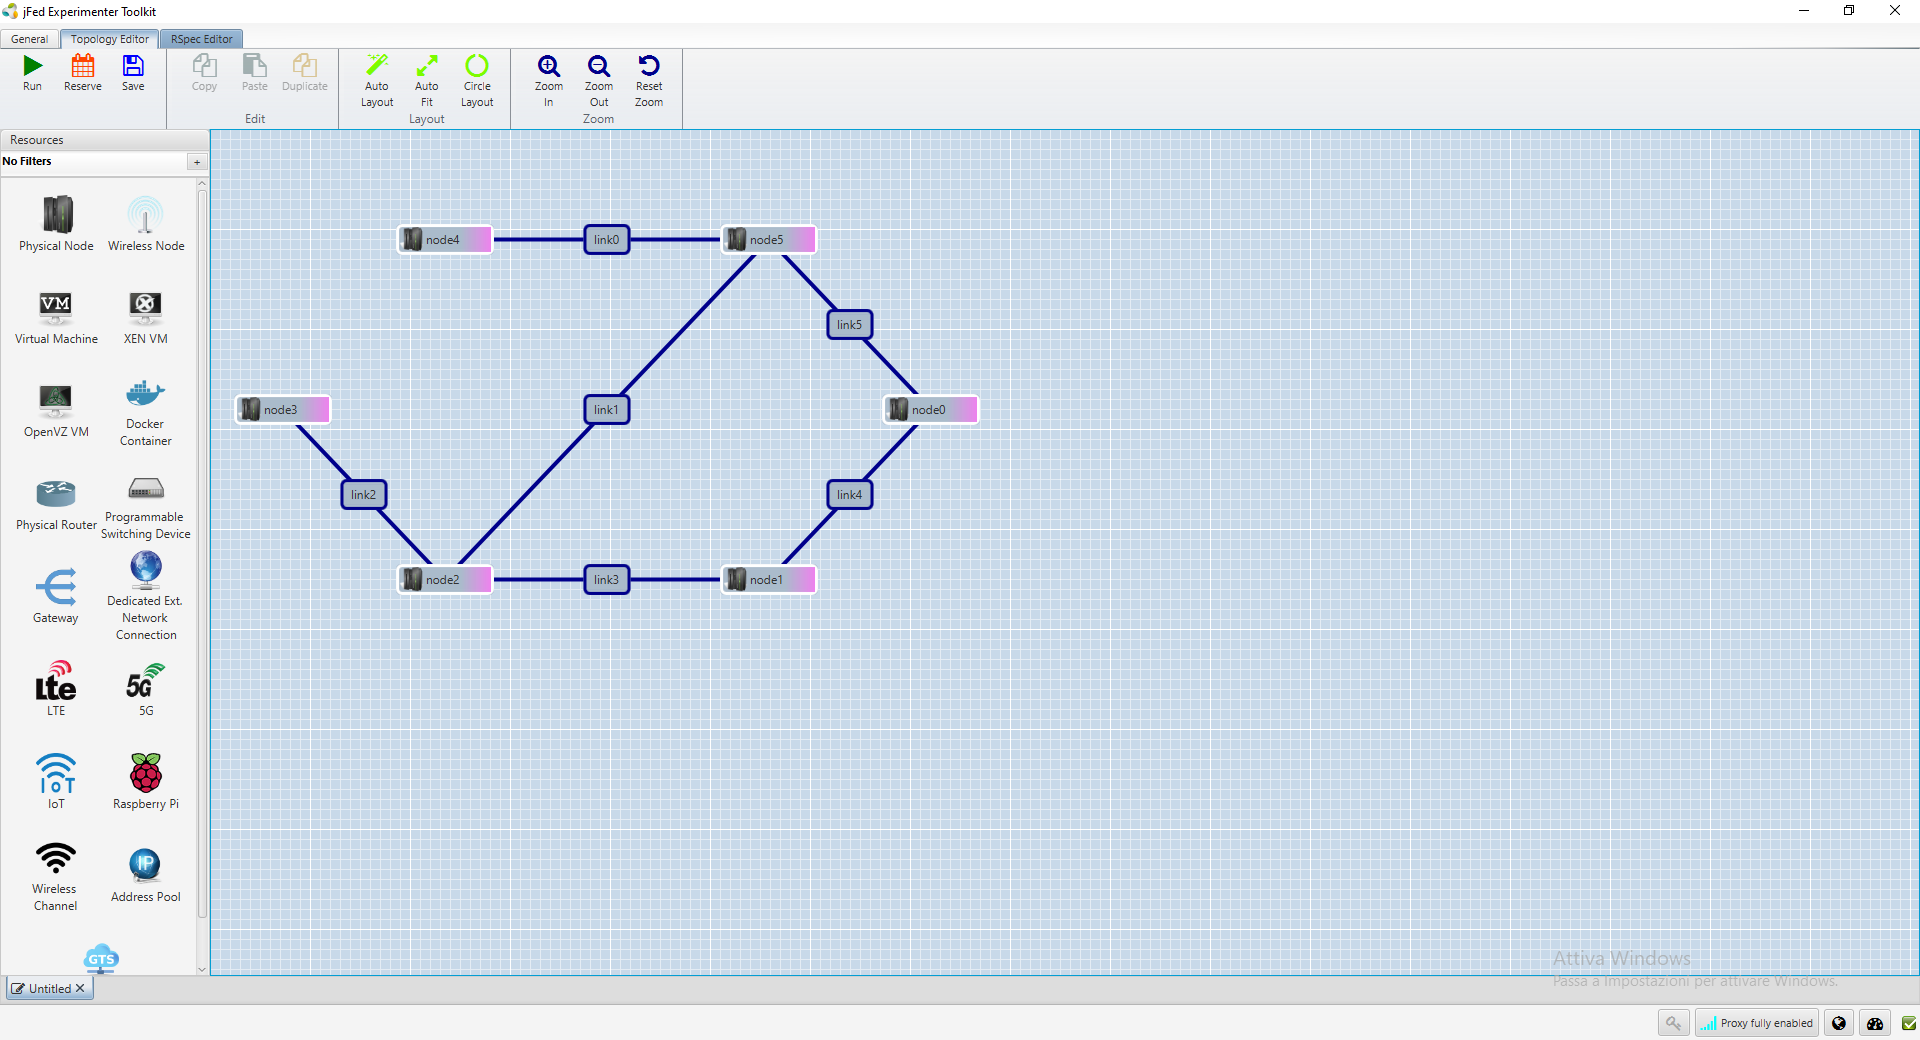
\includegraphics[width=13cm, height=7cm]{images/jfed.png}
            \caption {Esempio di esperimento su jfed}
            \label {fig:jfed}
    \end{center}
    \end {figure}
    
    
    I nodi utilizzati per la sperimentazione sono stati ospitati da:
    \begin{itemize}
        \item Virtual wall \cite {vw}, ospitato e gestito da imec e composto da due datacenter, Virtual Wall 1 (206 nodi) e Virtual Wall 2 (159 nodi). All'interno di LiSCIo i nodi di Virtual Wall sono stati sfruttati per imitare i nodi Cloud di una rete Fog
        \item CityLab \cite {cl}, un testbed destinato alla sperimentazione di reti wireless e 5G. Si trova nel centro della città di Anversa, in Belgio, e appartiene all'Università di Anversa/imec. Il testbed è situato nelle strade dentro e intorno al campus cittadino dell'Università di Anversa, in un'area di circa 0,5 km per 0,5 km. L'hardware attualmente è ospitato in 32 sedi con altre 22 pianificate. Ogni luogo ha il proprio gateway collegato alle case sulla strada o installato su un palo al di sopra di un tetto. Citylab punta sulla sperimentazione in rete per aumentare la maturità della connettività delle \emph{smart cities} \cite {clpdf} e per questo i suoi nodi sono stati usati all'interno di LiSCIo per imitare le risorse edge di una rete Fog.
    \end{itemize}